%% BioMed_Central_Tex_Template_v1.06
%%                                      %
%  bmc_article.tex            ver: 1.06 %
%                                       %

%%IMPORTANT: do not delete the first line of this template
%%It must be present to enable the BMC Submission system to
%%recognise this template!!

%%%%%%%%%%%%%%%%%%%%%%%%%%%%%%%%%%%%%%%%%
%%                                     %%
%%  LaTeX template for BioMed Central  %%
%%     journal article submissions     %%
%%                                     %%
%%          <8 June 2012>              %%
%%                                     %%
%%                                     %%
%%%%%%%%%%%%%%%%%%%%%%%%%%%%%%%%%%%%%%%%%


%%%%%%%%%%%%%%%%%%%%%%%%%%%%%%%%%%%%%%%%%%%%%%%%%%%%%%%%%%%%%%%%%%%%%
%%                                                                 %%
%% For instructions on how to fill out this Tex template           %%
%% document please refer to Readme.html and the instructions for   %%
%% authors page on the biomed central website                      %%
%% http://www.biomedcentral.com/info/authors/                      %%
%%                                                                 %%
%% Please do not use \input{...} to include other tex files.       %%
%% Submit your LaTeX manuscript as one .tex document.              %%
%%                                                                 %%
%% All additional figures and files should be attached             %%
%% separately and not embedded in the \TeX\ document itself.       %%
%%                                                                 %%
%% BioMed Central currently use the MikTex distribution of         %%
%% TeX for Windows) of TeX and LaTeX.  This is available from      %%
%% http://www.miktex.org                                           %%
%%                                                                 %%
%%%%%%%%%%%%%%%%%%%%%%%%%%%%%%%%%%%%%%%%%%%%%%%%%%%%%%%%%%%%%%%%%%%%%

%%% additional documentclass options:
%  [doublespacing]
%  [linenumbers]   - put the line numbers on margins

%%% loading packages, author definitions

%\documentclass[twocolumn]{bmcart}
% uncomment this for twocolumn layout and comment line below
\documentclass{bmcart}

%%% Load packages
%\usepackage{amsthm,amsmath}
%\RequirePackage{natbib}
\RequirePackage{hyperref}
\usepackage{etoolbox}
\usepackage[utf8x]{inputenc} %unicode support
\usepackage{graphicx}
\usepackage{tikz}
\usepackage{amsmath}
\usepackage{listings}
\usepackage{bera}
\usepackage{multirow}
\usepackage{fancyvrb}
\usepackage{soul}
%\usepackage[applemac]{inputenc} %applemac support if unicode package fails
%\usepackage[latin1]{inputenc} %UNIX support if unicode package fails


%%%%%%%%%%%%%%%%%%%%%%%%%%%%%%%%%%%%%%%%%%%%%%%%%
%%                                             %%
%%  If you wish to display your graphics for   %%
%%  your own use using includegraphic or       %%
%%  includegraphics, then comment out the      %%
%%  following two lines of code.               %%
%%  NB: These line *must* be included when     %%
%%  submitting to BMC.                         %%
%%  All figure files must be submitted as      %%
%%  separate graphics through the BMC          %%
%%  submission process, not included in the    %%
%%  submitted article.                         %%
%%                                             %%
%%%%%%%%%%%%%%%%%%%%%%%%%%%%%%%%%%%%%%%%%%%%%%%%%

%\def\includegraphic{}
%\def\includegraphics{}

  \makeatletter
  \patchcmd{\@addmarginpar}{\ifodd\c@page}{\ifodd\c@page\@tempcnta\m@ne}{}{}
  \makeatother
  \reversemarginpar
%%% Put your definitions there:
\startlocaldefs
  \newcommand{\comment}[2]{\hspace{0in}#2}
  \lstdefinelanguage{json}{
      basicstyle=\normalfont\ttfamily,
      numbersep=8pt,
      showstringspaces=false,
      breaklines=true,
      frame=lines,
      backgroundcolor=\color{white},
  }
\endlocaldefs


%%% Begin ...
\begin{document}

%%% Start of article front matter
\begin{frontmatter}

\begin{fmbox}
\dochead{Software}

%%%%%%%%%%%%%%%%%%%%%%%%%%%%%%%%%%%%%%%%%%%%%%
%%                                          %%
%% Enter the title of your article here     %%
%%                                          %%
%%%%%%%%%%%%%%%%%%%%%%%%%%%%%%%%%%%%%%%%%%%%%%

\title{A Powerful Scientific Names Parser ``gnparser'' Based on Parsing
Expression Grammars}

%%%%%%%%%%%%%%%%%%%%%%%%%%%%%%%%%%%%%%%%%%%%%%
%%                                          %%
%% Enter the authors here                   %%
%%                                          %%
%% Specify information, if available,       %%
%% in the form:                             %%
%%   <key>={<id1>,<id2>}                    %%
%%   <key>=                                 %%
%% Comment or delete the keys which are     %%
%% not used. Repeat \author command as much %%
%% as required.                             %%
%%                                          %%
%%%%%%%%%%%%%%%%%%%%%%%%%%%%%%%%%%%%%%%%%%%%%%

\author[
   addressref={aff1},
   corref={aff1},                       % id of corresponding address, if any
   email={mozzheri@illinois.edu}
]{\inits{DYM}\fnm{Dmitry Y.} \snm{Mozzherin}}
\author[                  % id's of addresses, e.g. {aff1,aff2}
   addressref={aff2},
   noteref={n1},% id's of article notes, if any
   email={alexander@myltsev.com}   % email address
]{\inits{AAM}\fnm{Alexander A.} \snm{Myltsev}}
\author[
   addressref={aff3},
   email={dpatterson.mbl@gmail.com}
]{\inits{DJP}\fnm{David J.} \snm{Patterson}}

%%%%%%%%%%%%%%%%%%%%%%%%%%%%%%%%%%%%%%%%%%%%%%
%%                                          %%
%% Enter the authors' addresses here        %%
%%                                          %%
%% Repeat \address commands as much as      %%
%% required.                                %%
%%                                          %%
%%%%%%%%%%%%%%%%%%%%%%%%%%%%%%%%%%%%%%%%%%%%%%

\address[id=aff1]{                     % unique id
  \orgname{University of Illinois},    % university, etc
  \street{1816 South Oak St.},         %
  \city{Champaign},                    % city
  \state{IL},
  \postcode{61820},
  \cny{US}                             % country
}

\address[id=aff2]{                     % unique id
  \orgname{IP Myltsev},                % university, etc
  \street{Kaslinskaya St.},            %
  \city{Chelyabinsk},                  % city
  \state{},
  \postcode{454084},
  \cny{Russia}                         % country
}

\address[id=aff3]{                     % unique id
  \orgname{University of Sydney},      % university, etc
  \city{Sydney},                       % city
  \cny{Australia}                      % country
}

%%%%%%%%%%%%%%%%%%%%%%%%%%%%%%%%%%%%%%%%%%%%%%
%%                                          %%
%% Enter short notes here                   %%
%%                                          %%
%% Short notes will be after addresses      %%
%% on first page.                           %%
%%                                          %%
%%%%%%%%%%%%%%%%%%%%%%%%%%%%%%%%%%%%%%%%%%%%%%

\begin{artnotes}
%\note{Sample of title note}     % note to the article
\note[id=n1]{Equal contributor} % note, connected to author
\end{artnotes}

\end{fmbox}% comment this for two column layout

%%%%%%%%%%%%%%%%%%%%%%%%%%%%%%%%%%%%%%%%%%%%%%
%%                                          %%
%% The Abstract begins here                 %%
%%                                          %%
%% Please refer to the Instructions for     %%
%% authors on http://www.biomedcentral.com  %%
%% and include the section headings         %%
%% accordingly for your article type.       %%
%%                                          %%
%%%%%%%%%%%%%%%%%%%%%%%%%%%%%%%%%%%%%%%%%%%%%%

\begin{abstractbox}

\begin{abstract} % abstract
  % Dima comment: Trying to make background much shorter here too
  \parttitle{Background}
  Linking biological data using scientific names creates tremendous
  opportunities for science. Variations in spellings of scientific names, many
  names for a taxon, one name for different taxons create a barrier to such
  linking. Breaking names into semantic elements is a necessary step to
  alleviate this problem.

  \parttitle{Results}
  We introduce Global Names Parser (\textit{gnparser}), a tool based on the
  Parsing Expression Grammar algorithm. The parser deals well with scientific
  name-strings of any complexity. It assigns semantic meaning to all elements
  within a scientific name-string (such as ranks, years of publication, names
  of authors, annotations, etc.). Global Names Parser is written in Scala, a
  Java Virtual Machine language. It performs with $\approx 99\%$ accuracy and
  processes 21.4 million name-strings/hour per CPU (73.4 million names/hour per
  4 CPUs). The \textit{gnparser} library is compatible with Scala, Java, R,
  Jython, and JRuby. The parser can be used as a command line application,
  socket server, web-app or RESTful http-service. It is released under an Open
  Source MIT license.

  \parttitle{Conclusions}
  Global Names Parser (\textit{gnparser}) is a fast, high precision tool for
  bioinformaticians working with scientific names. It can replace expensive and
  error-prone manual parsing and standardization of scientific names in many
  situations. Parsing increases the interoperability of distributed biological
  information from less than 15\% to ???\% by improving the matches among
  variant forms of the same scientific names.

\end{abstract}

%%%%%%%%%%%%%%%%%%%%%%%%%%%%%%%%%%%%%%%%%%%%%%
%%                                          %%
%% The keywords begin here                  %%
%%                                          %%
%% Put each keyword in separate \kwd{}.     %%
%%                                          %%
%%%%%%%%%%%%%%%%%%%%%%%%%%%%%%%%%%%%%%%%%%%%%%

\begin{keyword}
\kwd{biodiversity}
\kwd{scientific name}
\kwd{parser}
\end{keyword}

% MSC classifications codes, if any
%\begin{keyword}[class=AMS]
%\kwd[Primary ]{}
%\kwd{}
%\kwd[; secondary ]{}
%\end{keyword}

\end{abstractbox}
%
%\end{fmbox}% uncomment this for twcolumn layout

\end{frontmatter}

%%%%%%%%%%%%%%%%%%%%%%%%%%%%%%%%%%%%%%%%%%%%%%
%%                                          %%
%% The Main Body begins here                %%
%%                                          %%
%% Please refer to the instructions for     %%
%% authors on:                              %%
%% http://www.biomedcentral.com/info/authors%%
%% and include the section headings         %%
%% accordingly for your article type.       %%
%%                                          %%
%% See the Results and Discussion section   %%
%% for details on how to create sub-sections%%
%%                                          %%
%% use \cite{...} to cite references        %%
%%  \cite{koon} and                         %%
%%  \cite{oreg,khar,zvai,xjon,schn,pond}    %%
%%  \nocite{smith,marg,hunn,advi,koha,mouse}%%
%%                                          %%
%%%%%%%%%%%%%%%%%%%%%%%%%%%%%%%%%%%%%%%%%%%%%%

%%%%%%%%%%%%%%%%%%%%%%%%% start of article main body
% <put your article body there>

\section*{Conventions}

Throughout the paper we distinguish between two terms -- ``name'' and
``name-string''. Term ``name-strings'' represents a sequence of characters
(letters, numbers, punctuation, spaces, symbols). Term ``name'' is an entity
which points to a taxon. A name can be expressed by many name-strings, some are
well-formed and code compliant, and others are not (for example see
Table~\ref{table:carex}).  There are millions of scientific names and billions
of possible legitimate name-strings. In the paper we emphasize name-strings
with \textbf{bold}.

\section*{Background}

\marginpar{Dima:\\ Paddy and I decided on audience: Non-programmer people
working with bio-databases should be able to read title, abstract, background
without difficulties, understnd why parser is important for them, give paper to
programmers}

\marginpar{Dima: \\Alex and I decided on idea of the paper: we give most
advanced and still fast parser. It is fast and good because of combination of
Scala and PEG}


Biology is entering a ``Big Data'' age, where global and fast access to
knowledge becomes a reality. The names of organisms are invaluable in ``Big
Data'' biology because they make it possible to index, organize, and
interconnect distributed information \cite{Patterson2010}.  Nevertheless, use
of names for informatics purposes presents an array of problems. For example
there are several alternative spellings for a name (Table~\ref{table:carex}),
some names point to more than one taxon (homonyms), sometimes authorship in a
name-string is about a paper without a nomenclatural significance (chresonyms).

\begin{table}[!htb]
  \begin{center}

  \caption{Some legitimate versions of the scientific name for the Northern
    Bulrush or Singlespike sedge.  The genus (\textit{Carex}), species
    (\textit{scirpoidea}), and subspecies (\textit{convoluta}) may be annotated
    (var. subsp., and ssp.) or have the name of the original authority for the
    infraspecies (Kükenthal), the species (Michaux), the current infraspecific
    combination (Dunlop), sometimes abbreviated and with or without dates.
    Image courtesy of \cite{FNA2002}.}\label{table:carex}

    \begin{tabular}{| l | c |}
    \hline
    \textbf{Carex scirpoidea convoluta} &
    \multirow{26}{*}{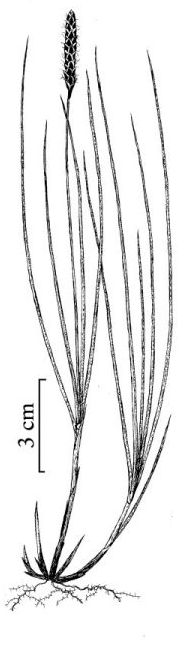
\includegraphics[scale=0.3]{images/carex.png}} \\
    & \\
    \textbf{Carex scirpoidea var. convoluta} & \\
    \textbf{Carex scirpoidea convoluta Kükenth.} & \\
    \textbf{Carex scirpoidea var. convoluta Kuk.} & \\
    \textbf{Carex scirpoidea var. convoluta Kük.} & \\
    \textbf{Carex scirpoidea var. convoluta Kükenth.} & \\
    \textbf{Carex scirpoidea var. convoluta Kükenthal} & \\
    \textbf{Carex scirpoidea Michx. var. convoluta Kük.} & \\
    \textbf{Carex scirpoidea Michx. var. convoluta Kükenth.} & \\
    \textbf{Carex scirpoidea Michaux var. convoluta Kükenthal} & \\
    & \\
    \textbf{Carex scirpoidea subsp. convoluta} & \\
    \textbf{Carex scirpoidea ssp. convoluta (Kük.) Dunlop} & \\
    \textbf{Carex scirpoidea subsp. convoluta (Kük.) Dunlop} & \\
    \textbf{Carex scirpoidea ssp. convoluta (Kukenth.) Dunlop} & \\
    \textbf{Carex scirpoidea subsp. convoluta (Kük.) D.A.Dunlop} & \\
    \textbf{Carex scirpoidea subsp. convoluta (Kük.) D.A. Dunlop} & \\
    \textbf{Carex scirpoidea Michx. ssp. convoluta (Kük.) Dunlop} & \\
    \textbf{Carex scirpoidea subsp. convoluta (Kuk.) D. A. Dunlop} & \\
    \textbf{Carex scirpoidea Michx. subsp. convoluta (Kük.) Dunlop} & \\
    \textbf{Carex scirpoidea Michx. ssp. convoluta (Kükenth.) Dunlop} & \\
    \textbf{Carex scirpoidea subsp. convoluta (Kükenthal) D.A. Dunlop} & \\
    \textbf{Carex scirpoidea Michx. subsp. convoluta (Kük.) D.A.Dunlop} & \\
    \textbf{Carex scirpoidea Michx. subsp. convoluta (Kük.) D.A. Dunlop} & \\
    \textbf{Carex scirpoidea subsp. convoluta (Kükenthal 1909) D.A. Dunlop 1998} & \\
    \hline
    \end{tabular}
  \end{center}
\end{table}

Name-strings example from Table~\ref{table:carex} clearly illustrates that
there is no universal obligatory way to spell scientific names. As a result
exact string matching links less than 15\% of entries in major data
environments \cite{Patterson:inpress-a}. Therefore it is necessary to reconcile
spelling variants with each other to connect them correctly.

Such reconciliation process involves linking name-strings into reconciliation
groups. If a biologist wants to do that s/he would mentally break name-strings
into elements (canonical form, authors, ranks etc.) or ``parse'' them. For
example to reconcile name-strings for a \textbf{Singlespike sedge} plant from
Table~\ref{table:carex} first a biologist would find that all of them have a
common ``canonical form'' -- \textbf{Carex scirpoidea convoluta}. Further
analysis of the name-strings would reveal two different reconciliation groups:

\begin{itemize}

  \item \textbf{Carex scirpoidea var. convoluta} description by
    \textbf{Kükenthal}

  \item \textbf{Carex scirpoidea subsp. convoluta} rank change by
    \textbf{Dunlop}.

\end{itemize}

A person familiar with botanical rules of nomenclature would do 24 name-strings
analysis with relative ease. However to scale such task to thousands and
millions of name-strings one would need an algorithmic way to find canonical
forms, ranks, authorships etc. One would need a sophisticated name parser!

Therefore a high qualilty parsing is quintessential for collecting large amount
of biological data, especially from multiple sources. We believe that a general
use parser should satisfy the following requirements to be up to the task:

\begin{enumerate}

  \item \textbf{High Quality.} A parser should be able to break names into their
    semantic elements to the same quality that can be achieved by a trained
    nomenclaturalist or better. Then parsing will be able to eliminate tedious
    and expensive manual work in many cases.

  \item \textbf{Global Scope.} A parser should be able to parse all types of
    scientific names, including the most complex name-strings -- hybrid
    formulae, multi-infraspecific names, names with multilevel authorships etc.
    No name-strings should be left behind, otherwise information attached to
    them will stay hidden from researchers.

  \item \textbf{Parsing Completeness.} All information included into a
    name-string is important, not only the canonical form. Authorship, year,
    rank information allow to distinguish homonyms, similar names, synonyms,
    spelling mistakes, chresonyms from each other, narrowing the search down to
    relevant information.

  \item \textbf{Speed.} For large-scale aggregators a parser needs to have a
    high throughput to collect data faster, to serve users with minimum delay,
    to reduce cost of hardware used for parsing.

  \item \textbf{Accessibility.} To be available to the widest possible audience
    a parser must be released as a stand-alone program. It has to have a
    good documentation, be able to work as a library, to function as a command
    line tool, as a tool with graphical interface, and to run as socket and
    RESTful services.

\end{enumerate}

These requirements became our design goals. Using a combination of Scala
programming language and Parsing Expression Grammars algorithm we created a
``gnparser'' project, and in ``Results and Discusson'' section we show how well
it fulfills these goals and describe ``prior art'' solutions of the problem.

\section*{Implementation}

The \textit{gnparser} project is entirely written in Scala. It supports two
major Scala versions: 2.10.3+ and 2.11.x. The code is organized into four
subprojects:

\begin{itemize}
  \item ``\textit{parser}'' contains core routines for parsing input string
  \item ``\textit{examples}'' contains usage samples for some popular
  programming languages: Java, Scala, Python, Ruby and R
  \item ``\textit{runner}'' contains code required to run ``\textit{parser}''
  from a command line as a standalone tool or to run it as a TCP/IP server
  \item ``\textit{web}'' contains a web application and a RESTful interface to
  ``\textit{parser}''
\end{itemize}

All subprojects but ``\textit{web}'' can run in JVM 1.6. ``\textit{web}''
requires JVM 1.8.

\textit{Parboiled2} is an Open Source project, which allowed us to extend
\comment{dima: would be good to add a few sentences to describe the extensions}
it to the needs of \textit{gnparser}.

\subsection*{parser}

``\textit{parser}'' contains components for successful parsing of a scientific
name: parsing grammar, abstract synthax tree (AST) composed of a scientific
name components, warnings and errors facilities, formatters:

\begin{itemize}

  \item \textit{normalizer} to standardize name-string.

  \item \textit{canonizer} to create canonical forms.

  \item \textit{JSON renderer} to convert output into JSON
    \cite{bray2014javascript}.

\end{itemize}

Typical ``parser'' is used as an external library. It provides parsing
facilities to other parts: language interoperability, command line tool, REST
and socket servers, etc.

``\textit{gnparser}'' accepts $String$ as input, and returns a $Result$.
$Result$ then can be converted to JSON containing the following useful
information:

\begin{itemize}
  \item $details$ contains JSON-representation of a parsed scientific name
  \item $quality\_warnings$ describes potential problems if names are not
    well-formed
  \item $quality$ depicts a quality level of a parsed name
  \item $positions$ maps positions of every word in a parsed name to
    a semantic meaning of the word
\end{itemize}

JSON schema can be found online \cite{gnparser-json}.

\subsection*{runner}

``\textit{runner}'' depends on ``\textit{parser}''. It provides functionality
of a command line tool and a socket server. Core part is the launch script
``\textit{gnparse}'' (for Linux/Mac and Windows) that creates JVM
instance and runs ``\textit{parser}'' on multiple threads against the input
provided via socket or file.

\subsection*{web}

``\textit{web}'' is a Play Framework \cite{wampler2011scala} application. It
depends on ``\textit{parser}'' library. ``\textit{web}'' allows to interact
with ``\textit{parser}'' via HTTP protocol. It aimed both with simple HTML
Figure~\ref{figure:webgui} and REST API interface.

\begin{figure}[htbp]
  \begin{center}
    \caption{
      Web Graphical User Interface
    }\label{figure:webgui}
    \vspace{5mm}

    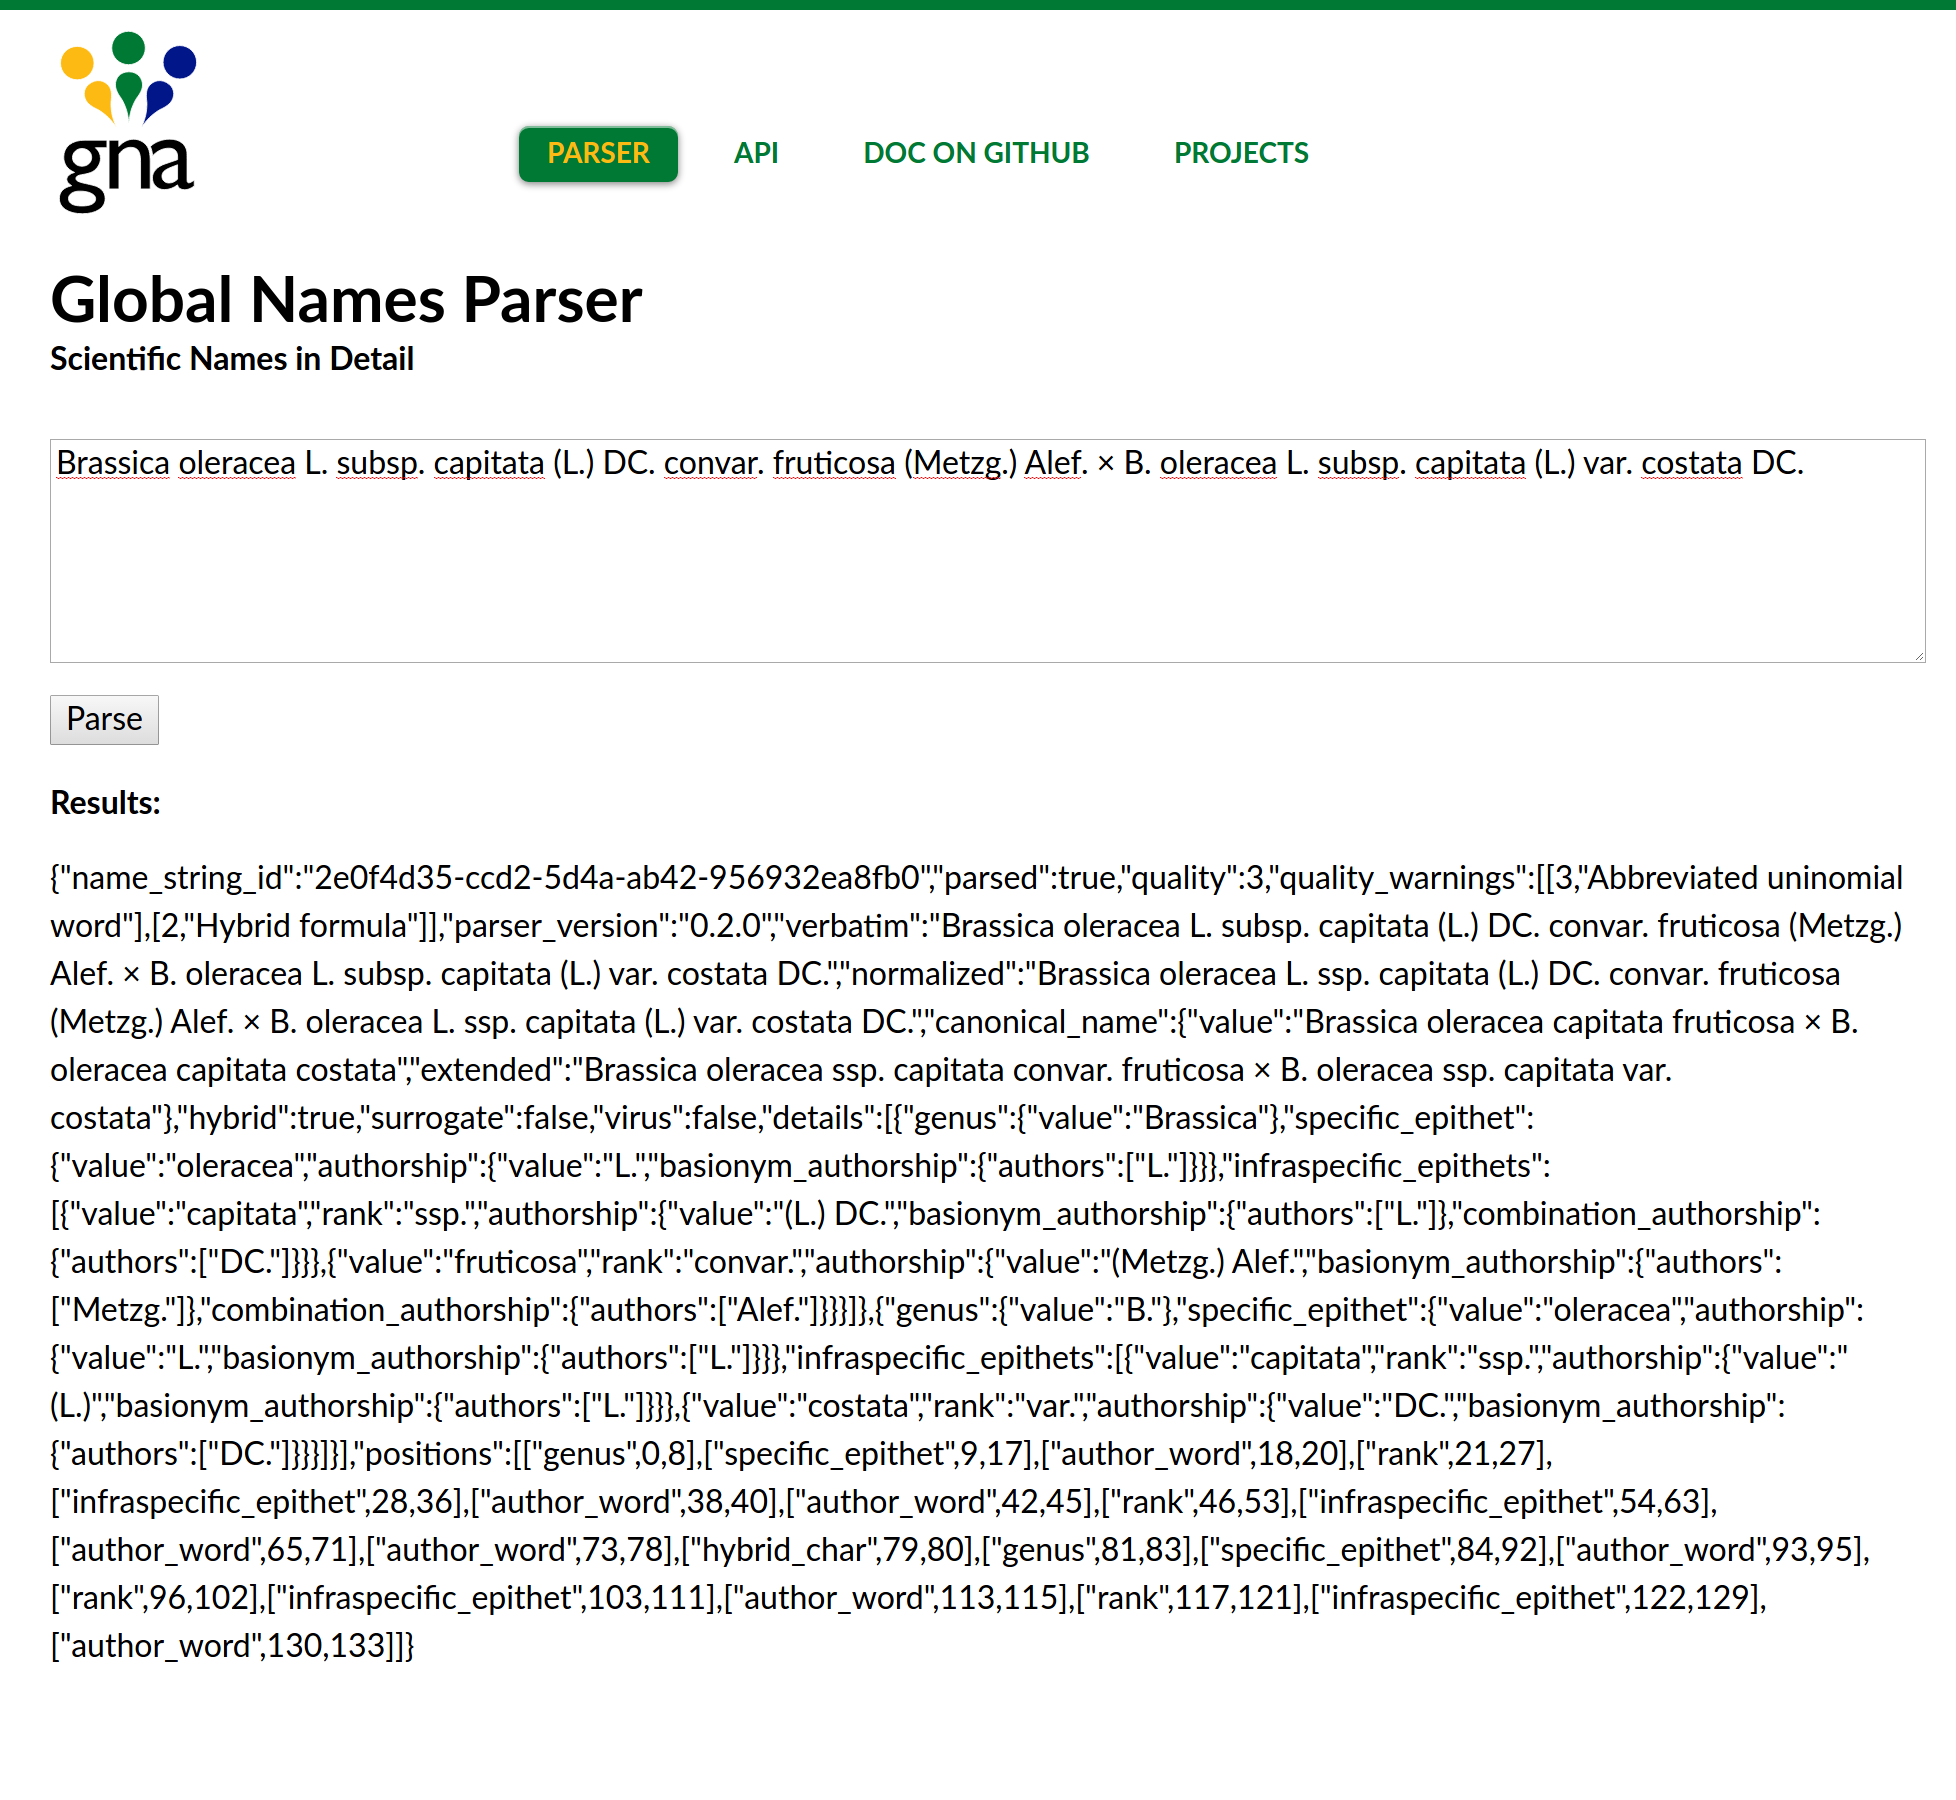
\includegraphics[scale=0.175]{images/web_gui.png}
  \end{center}
\end{figure}

Usage documentation is available at README file (see section ``Availability and
Requirements).

\subsection*{Installation}

``\textit{gnparser}'' is available for launch in three bundles:

\begin{itemize}
  \item A \textit{parser} artifact is provided via Maven central. Physically
    it is a relatively small jar file without external dependencies. The
    artifact can be referenced by a build system (Maven, Gradle, SBT, etc.) in
    another projects. Build system then provides resolution of required
    dependencies.

  \item Zip-archived ``fat jar'' is located at the project's GitHub repository.
    The jar contains \textit{gnparser} compiled files along with all
    necessary dependencies to launch it within JVM. The archive is also bundled
    with a launch script (for Windows, OS X and Linux) that can run command
    line interface to \textit{gnparser}.

  \item The project's Docker container is located at Docker hub. Docker
    provides an additional layer of abstraction and automation of
    operating-system-level virtualization on Linux. It can be thought as
    lightweight virtualization technology within same Linux OS process. When it
    is setup properly, everything -- starting from JVM and ending with Scala
    and SBT -- can be run with simple commands: pull Docker image from Hub, and
    then run socket or web server on a desired port.

\end{itemize}

\subsection*{Testing Methods}

Data for our tests (1,000 and 100,000 name-strings) were randomly chosen from
24 million name-strings of the Global Names Resolver \cite{resolver:gn}. These
resulting datasets consisted of strings acquired from a variety of data sources
and were a mixture of well-formed names, names with formatting and spelling
mistakes, and non-name strings misrepresented as names.

We compared performance of \textit{gnparser} with 2 other projects --
\textit{biodiversity} parser \cite{Boyle2013, biodiversity} (also developed by Global
Names), and GBIF \textit{name-parser} \cite{gbifNameParser}. For comparisons we
calculated $Precision$, $Recall$ and $Accuracy$ (as described below) using a
dataset consisted of 1000 name-strings. Another project we considered was
YASMEEN parser from iMarine project \cite{VandenBerghe2015}, however we found
that with our dataset it generated dramatically more mistakes than other
parsers ($Precision$ 0.534, $Recall$ 1.0, $F1$ 0.6962), and could not finish
full dataset without crashing, so we decided to exclude it from the tests.

To estimate quality for all parsers we needed to pick a feature which is common
for all three of them and is a good indicator of performance.  We decided to
use a combination of canonical form and terminal authorship.  Canonical form
represents the most stable elements of a name, while terminal authorship
corresponds to the authority of the most detailed classification element of the
name. For example in \textbf{Oriastrum lycopodioides Wedd.  var.  glabriusculum
Reiche} canonical form is \textbf{Oriastrum lycopodioides glabriusculum} and
terminal authorship is \textbf{Reiche}, not \textbf{Wedd.}.  Algorithms
necessary to select components of a canonical form of a name and to find the
terminal authorship are good indicators of a parsing quality.

When both the canonical form and the terminal authorship were determined
correctly we marked the result as true positive ($\text{tp}$).  If one or both
of them were determined incorrectly -- the result was marked a false positive
($\text{fp}$). Name-strings correctly discarded from parsing were marked as
true negatives ($\text{tn}$). False negatives ($\text{fn}$) were ``suitable''
name-strings which should be parsed, but were nevertheless discarded. The
following parameters where used for analysis:

$Accuracy$ -- a percentage of correctly determined results out of all results.
It is calculated as

\[Accuracy = \dfrac{\text{tp} + \text{tn}}
  {\text{tp} + \text{tn} + \text{fp} + \text{fn}}\]

$Precision$ -- a percentage of name-strings parsed correctly out of all
detected name-strings and is calculated as

\[Precision = \dfrac{\text{tp}}{(\text{tp} + \text{fp})}\]

$Recall$ -- a percentage of correctly detected name-strings out of all name-strings and is calculated as

\[Recall = \dfrac{\text{tp}}{(\text{tp} + \text{fn})}\]

$F1-measure$ is a balanced harmonic mean (where $Precision$ and $Recall$ have
the same weight). When both $Precision$ and $Recall$ vary, $F1-measure$ allows
to compare results nevertheless. It is calculated as

\[F1 = \dfrac{2 \times Precision \times Recall}{(Precision + Recall)}\]

Parsers can analyze the structure of a name-string, but they cannot determine
if a string is a ``real'' name -- it is out of the scope of parsers'
functionality.  For example in case of a name-string \textbf{"Example name Word
var. something Capitalized Words, 1900"}, canonical form \textbf{"Example
name something"} and terminal authorship \textbf{"Capitalized Words, 1900"}
would be considered a true positive.

Some names in the dataset were not well-formed. If a human could extract the
canonical form and the terminal authorship from them we did count them.
Examples of such name-strings are \textbf{"Bumetopia (bumetopia)
quadripunctata Breuning"} (low case subgenus), \textbf{"Campylium gollanii C.
M?ller ex Vohra 1970 [1972]"} (miscoded UTF-8 symbol and additional year in
square brackets), \textbf{"Myosorex muricauda (Miller, 1900)."} (period after
authorship).

It is important for parser to accurately distinguish between strings of
scientific names, names of viruses, surrogate names, and non-names. To find
out how well parsers distinguished strings which are not scientific names, we
calculated $Precision$ for discarded/non-parsed strings. If done correctly
not-parsed strings would include only names of viruses and non-scientific
names.

We processed 100,000 name-strings by each parser, and found that about 1000 of
them had been discarded as not-parseable. $Precision$ in this case showed
percentage of correctly discarded names.  We do not know $Recall$, as it was
not feasible to manually find it for 100,000 names. To get a glimpse on names
which had to be discarded, but were parsed instead we analysed intersections
and differences of the results between the three parsers.

To find out the throughput of parsing we used a computer with Intel i7-4930K
CPU (6 cores, 12 threads, at 3.4 GHz), 64GB of memory, and 250GB Samsung 840
EVO SSD, running Ubuntu version 14.04. Throughput was determined by processing
of 1,000,000 random name-strings from GNI.

To study effects of parallel execution on throughput we used
\textit{ParallelParser} class from \textit{biodiversity} parser and
\textit{gnparse} command line interface for \textit{gnparser}. For GBIF
\textit{name-parser} we created a thin wrapper with multi-threaded
capabilities \cite{gbifparser}.
\section*{Results and Discussion}

Until recently the problem of scientific name parsing had been addressed by
manual splitting of names into canonical form and the authorship part and
by using home-grown scripts based on regular expressions.

Manual approach of splitting names into 2 parts is expensive, slow, inflexible
and cannot elegantly deal with name-strings where authorship is present in the
middle of the name (for example \textbf{Carex scirpoidea Michx. subsp. convoluta
(Kük.) D.A.Dunlop}). The manual approach was never competitive for large scale
initiatives.

Another popular approach is to parse scientific names using regular language
implemented as regular expression \cite{aho1992foundations}. Regular expression
is a sequence of characters that describes a search pattern [REF].  For example
a regular expression ``[A-Z][a-z]\{2\}'' corresponds to a capitalized word from
3 letters like ``Zoo''. Examples of parsers based on regular expressions are
GBIF's \textit{name-parser} \cite{gbifNameParser}, \textit{YASMEEN}
\cite{VandenBerghe2015}.

Regular expression is a popular and powerful string matching tool, however it
does have well understood limits. For example regular expressions do not have
facilities to recursively refer parts of its own while parsing
\cite{yu1997handbook}. As a result it becomes very hard to deal with
recursively nested data structures.  Scientific names often have recursive
elements, most obvious example are hybrid formulae (for example
\textbf{Brassica oleracea L.  subsp.  capitata (L.) DC. convar. fruticosa
  (Metzg.) Alef.  $\times$ B. oleracea L. subsp. capitata (L.) var.  costata
DC.}). That makes approaches to scientific names parsing built on regular
expressions impractical for complex name-strings.

Moreover, most of the regular expression software tools are ``black boxes''.
They allow very little interaction with the parsing process, and information
about parsing context is limited. A developer cannot call a procedure during a
parsing event. As a result it is hard/impossible to implement and maintain such
concepts as error recovery, detailed warnings and errors description.

We wanted to find an algorithm that is able to deal with names of broader
complexity and gives more flexibility than a regular expression approach.

\subsection*{Adoption of Parsing Expression Grammars}

We chose Parsing Expression Grammar (PEG) \cite{Ford2004} as an underlying
technology. PEG is an alternative to regular expression method for describing a
synthax of scientific names. We think PEG is better for our goals for the
following reasons:

\begin{itemize}

  \item PEG is well suited for texts with recursive synthax.

  \item scientific names' synthax is formalized enough to be closer to strict
    algebraic description rather than to a natural language. Inconsistencies
    and ambiguities in scientific names are relatively rare due to adherence to
    nomenclatural codes.

  \item typical scientific name-string is short enough to avoid potentially
    bad computational complexity and memory consumption

  \item programming a parser is easier than with regular
    expressions because PEG allows to compose parsing rules in a clear domain
    specific language

  \item Such domain specific language allows great flexibility for logic within
    the rules, for example for reporting errors in name-strings.

\end{itemize}

In 2008 we created a specialized parsing library \textit{biodiversity}
\cite{biodiversity} written in Ruby and based on PEG. We used an excellent
\textit{TreeTop} Ruby library \cite{treetop} as an underlying PEG
implementation.

We found that PEG approach allowed us to deal with complex scientific names
gracefully. Also PEG gave us enough flexibility to incorporate edge cases and
common mistakes detection during the parsing process. The library
\textit{biodiversity} enjoyed noticeable popularity. At a time of writing it
had been downloaded more than 150,000 times \cite{bdiv-downloads}, it is used
by many taxon name resolution projects (for example by Encyclopedia of Life
\cite{eol}, Canadian Register of Marine Species (CARMS) \cite{carms}, the
iPlant TNRS \cite{iplant}, World Registry of Marine Species (WoRMS)
\cite{worms}.  According to BioRuby statistics \textit{biodiversity}, at the
time of writing, had been the most popular bio-library in Ruby language
\cite{biogems}.

We consider \textit{biodiversity} parser library to be a working prototype -- a
playground which allowed us to identify parsing problems and implement
solutions for them. We also found that PEG is very well suited for scientific
names parsing.

\subsection*{Adoption of Scala}

The parser \textit{biodiversity} faced performance and scalability issues
inherited from Ruby design. Ruby is one of the best languages for rapid
prototyping. The drawback is that it is an interpreted dynamic language with
originally single-threaded runtime in virtual machine. We needed to move
forward to an environment with the following properties:

\begin{itemize}
    \item mature technology
    \item multi-threaded, with high performance and scalability
    \item active community with open-source friendly culture
    \item a wide range of libraries: utilities, web frameworks, etc.
    \item mature development environment: IDEs, testings frameworks,
    debuggers, profilers
    \item technologies for search and cluster computations
    \item interoperability with languages used in scientific community (R,
    Python, Matlab)
    \item natural support of domain specific languages embedded in hosted
    language
\end{itemize}

While many of the properties are true for Ruby as well, others are lacking in
the language. In 2015 we decided to use everything we learned from
\textit{biodiversity}, and found technologies to fulfil all requirements: Java
virtual machine, Scala programming language \cite{odersky2004overview}, and
\textit{parboiled2} library \cite{parboiled2}. There is an alternative to
\textit{parboiled2} -- the Scala parser combinators library
\cite{moors2008parser}. However the library has known performance and memory
issues so \textit{parboiled2} was a natural choice.

Functional programming features of Scala language help to avoid use of
external grammar generators, allowing to write a grammar directly in Scala
using higher-order combinators. \textit{Parboiled2} has a grammar rule domain
specific language that is macro-translated
\cite{Burmako:2013:SML:2489837.2489840} to a high performance code.

Using Scala and \textit{parboiled2} we wrote \textit{gnparser} -- a
completely new parser -- and achieved significant boost in speed, scalability
and portability of the library. In this manuscript we describe features,
performance and discuss future enhancements of this new parser.

We discuss \textit{gnparser}, GBIF \textit{name-pasrser} and
\textit{biodiversity} parser from the point of the 5 requirements mentioned
earlier in the Background section:

\begin{enumerate}
  \item High Quality Parsing
  \item Global Scope
  \item Parsing Completeness
  \item Speed
  \item Accessibility
\end{enumerate}

\subsection*{High Quality Parsing}

High quality parsing is probably the most important out of the 5 requirements.
We tested \textit{gnparser} together with 2 other parsing projects. To our
knowledge these three represent state of the art for parsing biological
scientific names. GBIF \textit{name-parser} uses regular expressions approach,
while \textit{gnparser} and \textit{biodiversity} parser use PEG approach.
Results for our quality measurements are shown in Table~\ref{table:precision}.

When data contain large proportion of true negatives ($\text{tn}$) $Accuracy$
is not a good measure, as it would favor algorithms which distinguish negative
results, rather than finding positive ones. However by manual checking we
found that our datasets had only $\approx1\%$ of non-scientific names, true
negatives were rare and had very little influence on results. $Recall$ for all
parsers was very high, which means false negatives had an insignificant
influence on results as well. We hold that $Accuracy$ is the best measure for
our tests and is sufficient to compare quality for all cases.

Altogether we find that all 3 parsers performed very well with $Accuracy$
values higher than $95\%$. Both \textit{gnparser} and \textit{biodiversity}
parser were approaching 99\% mark\st{, that is production
quality}\marginpar{Dima: \\removed it to avoid explanation what we consider
production quality, as others might have different ideas}. Moreover, most of
the false positives came from name-strings with mistakes. For example for 1000
name-string data set, out of 11 false positives for \textit{gnparser} only 2
(the upper two) were well-formed names:

\vspace{0.5cm}

\begin{verbatim}
    Eucalyptus subser. Regulares Brooker
    Jacquemontia spiciflora (Choisy) Hall. fil.

    Acanthocephala declivis variety guianensis Osborn, 1904
    Atysa (?) frontalis
    Bumetopia (bumetopia) quadripunctata Breuning, 1950
    Cyclotella kã¼tzingiana Thwaites
    Elaphidion (romaleum) tæniatum Leconte, 1873
    Hieracium nobile subsp. perclusum (Arv. -Touv. ) O. Bolòs & Vigo
    Leptomitus vitreus (Roth) Agardh{?}
    Myosorex muricauda (Miller, 1900).
    Papillaria amblyacis (M<81>ll.Hal.) A.Jaeger
\end{verbatim}

\vspace{0.5cm}

As it is seen from the name-strings above we do expect parsers to deal with
mistakes, annotations, and Unicode characters miscodings. To alert users,
\textit{gnparser} generates warnings for each found problem in a name-string.
The other parsers do not have this feature.

When parsers reach $\approx80\%$ $Accuracy$, they hit a ``long tail'' of
problems where each particular type of a problem  is rare, yet every new manual
test against 1,000-10,000 name-strings reveals new issues.  Examples of these
challenges are given elsewhere \cite{Patterson:inpress-a}. For all three
parsers, developers performed a meticulous task of adding one rare case after
another to the list of problems and finding ways to incorporate solutions. That
is, parsers need to be subject to continuous improvement. The problems found
during preparation of this paper are being addressed in the next version of
\textit{gnparser} as well. As the parsing rules improve, we believe that
\textit{gnparser} can reach $>99.5\%$ $Accuracy$ without diminishing $Recall$.

As we incorporate new rules to increase $Recall$, we have to consider the risks
of reducing $Precision$ by introducing new false positives. For example GBIF
\textit{name-parser} allows the genus element of a name-string to start with a
lowercase character. As a result the name-strings below were parsed as if they
were scientific names, while other parsers ignored them:

\vspace{0.5cm}

\begin{verbatim}
    acid mine drainage metagenome
    agricultural soil bacterium CRS5639T18-1
    agricultural soil bacterium SC-I-8
    algal symbiont of Cladonia variegata MN075
    alpha proteobacterium AP-24
    anaerobic bacterium ANA No.5
    anoxygenic photosynthetic bacterium G16
    archaeon enrichment culture clone AOM-SR-A23
    bacterium endosymbiont of Plateumaris fulvipes
    bacterium enrichment culture DGGE band 61_3_FG_L
    barley rhizosphere bacterium JJ-220
    bovine rumen bacterium niuO17
\end{verbatim}

\vspace{0.5cm}

Solutions like these might increase $Recall$ with certain low-quality datasets,
but they also may decrease $Precision$ with other datasets. When dealing with
``dirty'' datasets containing predictable problems, we find the best solution is
to include a ``preparser'' script which ``normalizes'' known problems and then
apply a high quality parser to the result.  As an example, a recent study of
name-strings in DRYAD revealed a large number of instances where elements of
scientific names had been concatenated with an interpolated character such
as `\_’ (e.g. ``Homo\_sapiens'' and ``Pinoyscincus\_jagori\_grandis'')
\cite{Patterson:inpress-a}.

Our testing also revealed differences between regular expressions and PEG
approaches. Both can achieve high quality results with canonical forms, but the
regular expressions approach is less suitable for more complex name-strings.
The reason for this is the recursive nature of scientific names.  It is
relatively straightforward to parse ``simple'' name-strings with regular
expressions, but the recursive nature of some names-strings present greater
problems that at some point become unsurmountable.

\subsection*{Global Scope}

If we want to truly connect biological data using scientific names, no
name-strings should be left behind, no matter how complex they are. During our
testing we found that $Accuracy$ of GBIF \textit{name-parser} was negatively
affected by not dealing with hybrid formulae and infrasubspecific names (names
with more then one infraspecific epithet). Regular expressions do not support
recursion -- the more complex names are, the harder it becomes to parse them.
For example the following names were not supported by GBIF
\textit{name-parser}:

\vspace{0.5cm}

\begin{verbatim}
    Crataegus chlorosarca subtaxon pubescens E.L.Wolf
    Erigeron peregrinus ssp.callianthemus var. eucallianthemus
    Salvelinus fontinalis x Salmo gairdneri
    Echinocereus fasciculatus var. bonkerae × E. fasciculatus
      var. fasciculatus
\end{verbatim}

\vspace{0.5cm}

We use PEG approach because it supports nesting parsing rules within each
other, and creates progressively more and more complex rules. The first rule
just defines a space between words, the last rule defines hybrid
formulas.  Such support for recursion allows \textit{gnparser} to handle full
spectrum of scientific names.

\begin{table}[htb]
  \begin{center}
    \caption{Precision/Recall for processed by parsers 1000
    name-strings}\label{table:precision}
    \resizebox{10cm}{!} {
    \begin{tabular}{|l|*{3}{l}|}
      \hline
                             & gnparser & gbif-parser & biodiversity \\
      \hline
      \textit{True Positive} & 976      & 955         & 971          \\
      \textit{True Negative} & 13       & 12          & 13           \\
      \textit{False Positive}& 11       & 32          & 16           \\
      \textit{False Negative}& 0        & 1           & 0            \\
      \textit{Precision}     & 0.9888551& 0.967578    & 0.9837893    \\
      \textit{Recall}        & 1.0      & 0.998954    & 1.0          \\
      \textit{F1}            & 0.9943963& 0.983016    & 0.9918284    \\
      \textit{Accuracy}      & 0.989    & 0.967       & 0.984        \\
      \hline
    \end{tabular}
    }
  \end{center}
\end{table}

\begin{table}[htb]
  \begin{center}
    \caption{Precision for discarded by parsers names, out of 100 000
    name-strings}\label{table:unparsed}
    \resizebox{10cm}{!} {
    \begin{tabular}{| l | *{3}{l} |}
      \hline
                              & gnparser & gbif-parser & biodiversity \\
      \hline
      \textit{Total discarded}& 1131     & 1082        & 1161         \\
      \textit{True Positive}  & 1129     & 940         & 1152         \\
      \textit{False Positive} & 2        & 142         & 9            \\
      \textit{Precision}      & 0.998231 & 0.868761    & 0.9922481    \\
      \hline
    \end{tabular}
  }
  \end{center}
\end{table}

\begin{figure}[htbp]
  \begin{center}
    \caption{
      Names parsed per second by GN, GBIF and Biodiversity parsers
      (running on 1-12 parallel threads).
    }\label{figure:throughput}
    \vspace{0.5cm}
    \begin{tabular}{| l | *{3}{r} | c c c |}
      \hline
      \multirow{1}{*}Threads & gnparser & gbif-paser & biodiversity
      & \multicolumn{3}{c |}{Ratio} \\
      \cline{5-7}
      & & & & gn & gbif & bio \\
      \hline
      1  & 5944  & 6389  & 1111 & 1 & 1.07 & 0.19 \\
      2  & 11416 & 12638 & 1722 & 1 & 1.11 & 0.14 \\
      4  & 20500 & 21994 & 2556 & 1 & 1.07 & 0.12 \\
      8  & 24805 & 30972 & 2777 & 1 & 1.25 & 0.11 \\
      12 & 26055 & 31833 & 2527 & 1 & 1.22 & 0.10 \\
      \hline
    \end{tabular}
    % Created by tikzDevice version 0.9 on 2015-12-21 16:35:00
% !TEX encoding = UTF-8 Unicode
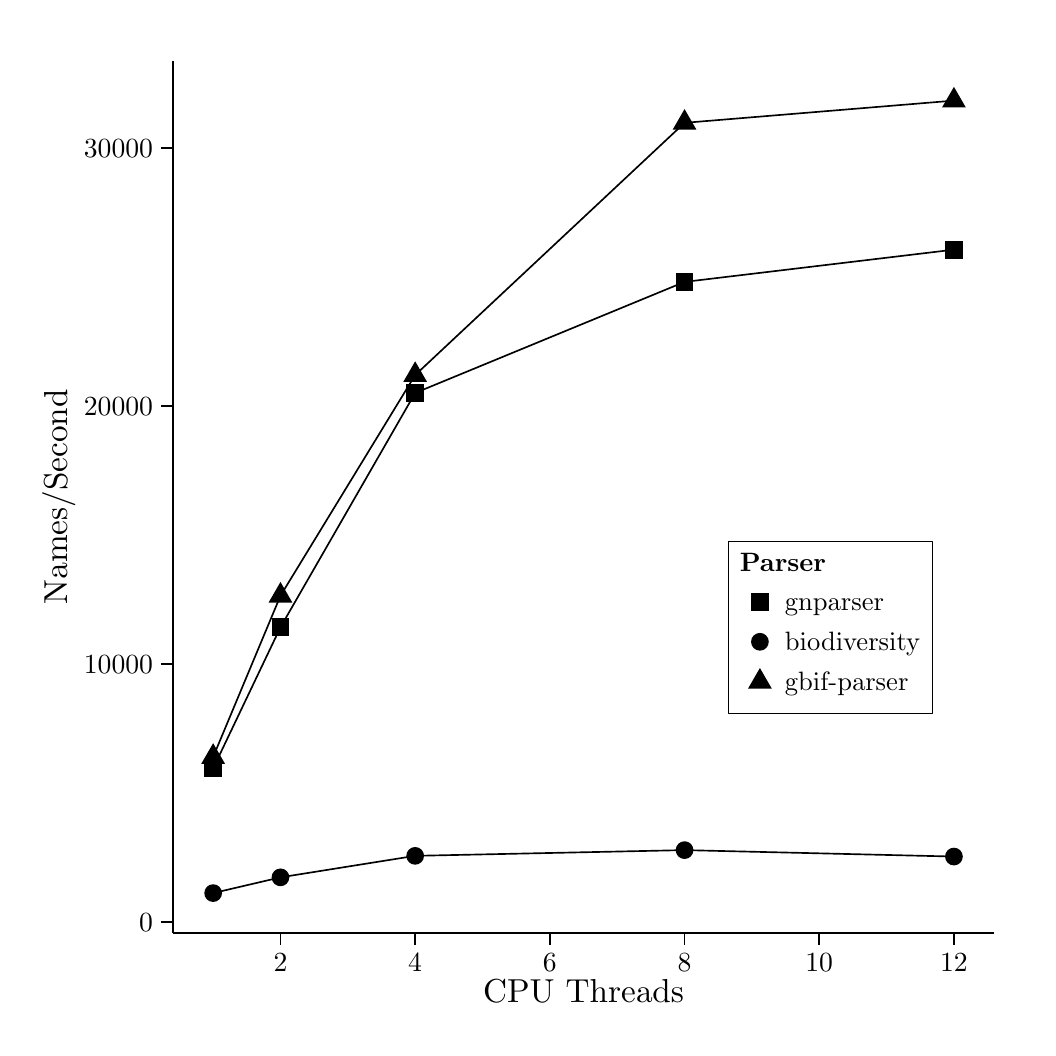
\begin{tikzpicture}[x=1pt,y=1pt]
\definecolor{fillColor}{RGB}{255,255,255}
\path[use as bounding box,fill=fillColor,fill opacity=0.00] (0,0) rectangle (361.35,361.35);
\begin{scope}
\path[clip] (  0.00,  0.00) rectangle (361.35,361.35);
\definecolor{drawColor}{RGB}{255,255,255}
\definecolor{fillColor}{RGB}{255,255,255}

\path[draw=drawColor,line width= 0.6pt,line join=round,line cap=round,fill=fillColor] (  0.00,  0.00) rectangle (361.35,361.35);
\end{scope}
\begin{scope}
\path[clip] ( 52.42, 34.31) rectangle (349.30,349.30);
\definecolor{fillColor}{RGB}{255,255,255}

\path[fill=fillColor] ( 52.42, 34.31) rectangle (349.30,349.30);
\definecolor{drawColor}{RGB}{255,255,255}

\path[draw=drawColor,line width= 0.6pt,line join=round] ( 52.42, 38.27) --
	(349.30, 38.27);

\path[draw=drawColor,line width= 0.6pt,line join=round] ( 52.42,131.48) --
	(349.30,131.48);

\path[draw=drawColor,line width= 0.6pt,line join=round] ( 52.42,224.69) --
	(349.30,224.69);

\path[draw=drawColor,line width= 0.6pt,line join=round] ( 52.42,317.90) --
	(349.30,317.90);

\path[draw=drawColor,line width= 0.6pt,line join=round] ( 91.35, 34.31) --
	( 91.35,349.30);

\path[draw=drawColor,line width= 0.6pt,line join=round] (140.02, 34.31) --
	(140.02,349.30);

\path[draw=drawColor,line width= 0.6pt,line join=round] (188.69, 34.31) --
	(188.69,349.30);

\path[draw=drawColor,line width= 0.6pt,line join=round] (237.36, 34.31) --
	(237.36,349.30);

\path[draw=drawColor,line width= 0.6pt,line join=round] (286.03, 34.31) --
	(286.03,349.30);

\path[draw=drawColor,line width= 0.6pt,line join=round] (334.70, 34.31) --
	(334.70,349.30);
\definecolor{drawColor}{RGB}{0,0,0}

\path[draw=drawColor,line width= 0.6pt,line join=round] ( 67.02, 48.63) --
	( 91.35, 54.32) --
	(140.02, 62.09) --
	(237.36, 64.16) --
	(334.70, 61.83);

\path[draw=drawColor,line width= 0.6pt,line join=round] ( 67.02, 97.82) --
	( 91.35,156.08) --
	(140.02,235.82) --
	(237.36,326.96) --
	(334.70,334.99);

\path[draw=drawColor,line width= 0.6pt,line join=round] ( 67.02, 93.68) --
	( 91.35,144.69) --
	(140.02,229.35) --
	(237.36,269.48) --
	(334.70,281.13);
\definecolor{fillColor}{RGB}{0,0,0}

\path[fill=fillColor] ( 63.82, 90.48) --
	( 70.22, 90.48) --
	( 70.22, 96.88) --
	( 63.82, 96.88) --
	cycle;

\path[fill=fillColor] ( 88.15,141.48) --
	( 94.55,141.48) --
	( 94.55,147.89) --
	( 88.15,147.89) --
	cycle;

\path[fill=fillColor] (136.82,226.15) --
	(143.22,226.15) --
	(143.22,232.55) --
	(136.82,232.55) --
	cycle;

\path[fill=fillColor] (234.16,266.28) --
	(240.56,266.28) --
	(240.56,272.68) --
	(234.16,272.68) --
	cycle;

\path[fill=fillColor] (331.50,277.93) --
	(337.90,277.93) --
	(337.90,284.33) --
	(331.50,284.33) --
	cycle;

\path[fill=fillColor] ( 67.02,102.80) --
	( 71.33, 95.33) --
	( 62.71, 95.33) --
	cycle;

\path[fill=fillColor] ( 91.35,161.06) --
	( 95.66,153.59) --
	( 87.04,153.59) --
	cycle;

\path[fill=fillColor] (140.02,240.80) --
	(144.33,233.33) --
	(135.71,233.33) --
	cycle;

\path[fill=fillColor] (237.36,331.94) --
	(241.67,324.47) --
	(233.05,324.47) --
	cycle;

\path[fill=fillColor] (334.70,339.96) --
	(339.01,332.50) --
	(330.39,332.50) --
	cycle;

\path[fill=fillColor] ( 67.02, 48.63) circle (  3.20);

\path[fill=fillColor] ( 91.35, 54.32) circle (  3.20);

\path[fill=fillColor] (140.02, 62.09) circle (  3.20);

\path[fill=fillColor] (237.36, 64.16) circle (  3.20);

\path[fill=fillColor] (334.70, 61.83) circle (  3.20);
\end{scope}
\begin{scope}
\path[clip] (  0.00,  0.00) rectangle (361.35,361.35);
\definecolor{drawColor}{RGB}{0,0,0}

\path[draw=drawColor,line width= 0.6pt,line join=round] ( 52.42, 34.31) --
	( 52.42,349.30);
\end{scope}
\begin{scope}
\path[clip] (  0.00,  0.00) rectangle (361.35,361.35);
\definecolor{drawColor}{RGB}{0,0,0}

\node[text=drawColor,anchor=base east,inner sep=0pt, outer sep=0pt, scale=  1.00] at ( 45.30, 34.83) {0};

\node[text=drawColor,anchor=base east,inner sep=0pt, outer sep=0pt, scale=  1.00] at ( 45.30,128.04) {10000};

\node[text=drawColor,anchor=base east,inner sep=0pt, outer sep=0pt, scale=  1.00] at ( 45.30,221.25) {20000};

\node[text=drawColor,anchor=base east,inner sep=0pt, outer sep=0pt, scale=  1.00] at ( 45.30,314.46) {30000};
\end{scope}
\begin{scope}
\path[clip] (  0.00,  0.00) rectangle (361.35,361.35);
\definecolor{drawColor}{RGB}{0,0,0}

\path[draw=drawColor,line width= 0.6pt,line join=round] ( 48.15, 38.27) --
	( 52.42, 38.27);

\path[draw=drawColor,line width= 0.6pt,line join=round] ( 48.15,131.48) --
	( 52.42,131.48);

\path[draw=drawColor,line width= 0.6pt,line join=round] ( 48.15,224.69) --
	( 52.42,224.69);

\path[draw=drawColor,line width= 0.6pt,line join=round] ( 48.15,317.90) --
	( 52.42,317.90);
\end{scope}
\begin{scope}
\path[clip] (  0.00,  0.00) rectangle (361.35,361.35);
\definecolor{drawColor}{RGB}{0,0,0}

\path[draw=drawColor,line width= 0.6pt,line join=round] ( 52.42, 34.31) --
	(349.30, 34.31);
\end{scope}
\begin{scope}
\path[clip] (  0.00,  0.00) rectangle (361.35,361.35);
\definecolor{drawColor}{RGB}{0,0,0}

\path[draw=drawColor,line width= 0.6pt,line join=round] ( 91.35, 30.04) --
	( 91.35, 34.31);

\path[draw=drawColor,line width= 0.6pt,line join=round] (140.02, 30.04) --
	(140.02, 34.31);

\path[draw=drawColor,line width= 0.6pt,line join=round] (188.69, 30.04) --
	(188.69, 34.31);

\path[draw=drawColor,line width= 0.6pt,line join=round] (237.36, 30.04) --
	(237.36, 34.31);

\path[draw=drawColor,line width= 0.6pt,line join=round] (286.03, 30.04) --
	(286.03, 34.31);

\path[draw=drawColor,line width= 0.6pt,line join=round] (334.70, 30.04) --
	(334.70, 34.31);
\end{scope}
\begin{scope}
\path[clip] (  0.00,  0.00) rectangle (361.35,361.35);
\definecolor{drawColor}{RGB}{0,0,0}

\node[text=drawColor,anchor=base,inner sep=0pt, outer sep=0pt, scale=  1.00] at ( 91.35, 20.31) {2};

\node[text=drawColor,anchor=base,inner sep=0pt, outer sep=0pt, scale=  1.00] at (140.02, 20.31) {4};

\node[text=drawColor,anchor=base,inner sep=0pt, outer sep=0pt, scale=  1.00] at (188.69, 20.31) {6};

\node[text=drawColor,anchor=base,inner sep=0pt, outer sep=0pt, scale=  1.00] at (237.36, 20.31) {8};

\node[text=drawColor,anchor=base,inner sep=0pt, outer sep=0pt, scale=  1.00] at (286.03, 20.31) {10};

\node[text=drawColor,anchor=base,inner sep=0pt, outer sep=0pt, scale=  1.00] at (334.70, 20.31) {12};
\end{scope}
\begin{scope}
\path[clip] (  0.00,  0.00) rectangle (361.35,361.35);
\definecolor{drawColor}{RGB}{0,0,0}

\node[text=drawColor,anchor=base,inner sep=0pt, outer sep=0pt, scale=  1.20] at (200.86,  9.03) {CPU Threads};
\end{scope}
\begin{scope}
\path[clip] (  0.00,  0.00) rectangle (361.35,361.35);
\definecolor{drawColor}{RGB}{0,0,0}

\node[text=drawColor,rotate= 90.00,anchor=base,inner sep=0pt, outer sep=0pt, scale=  1.20] at ( 14.29,191.81) {Names/Second};
\end{scope}
\begin{scope}
\path[clip] (  0.00,  0.00) rectangle (361.35,361.35);
\definecolor{drawColor}{RGB}{0,0,0}
\definecolor{fillColor}{RGB}{255,255,255}

\path[draw=drawColor,line width= 0.3pt,line join=round,line cap=round,fill=fillColor] (253.09,113.49) rectangle (326.76,175.63);
\end{scope}
\begin{scope}
\path[clip] (  0.00,  0.00) rectangle (361.35,361.35);
\definecolor{drawColor}{RGB}{0,0,0}

\node[text=drawColor,anchor=base west,inner sep=0pt, outer sep=0pt, scale=  0.96] at (257.36,164.73) {\bfseries Parser};
\end{scope}
\begin{scope}
\path[clip] (  0.00,  0.00) rectangle (361.35,361.35);
\definecolor{drawColor}{RGB}{255,255,255}
\definecolor{fillColor}{RGB}{255,255,255}

\path[draw=drawColor,line width= 0.6pt,line join=round,line cap=round,fill=fillColor] (257.36,146.67) rectangle (271.82,161.12);
\end{scope}
\begin{scope}
\path[clip] (  0.00,  0.00) rectangle (361.35,361.35);
\definecolor{fillColor}{RGB}{0,0,0}

\path[fill=fillColor] (261.39,150.69) --
	(267.79,150.69) --
	(267.79,157.09) --
	(261.39,157.09) --
	cycle;
\end{scope}
\begin{scope}
\path[clip] (  0.00,  0.00) rectangle (361.35,361.35);
\definecolor{drawColor}{RGB}{255,255,255}
\definecolor{fillColor}{RGB}{255,255,255}

\path[draw=drawColor,line width= 0.6pt,line join=round,line cap=round,fill=fillColor] (257.36,132.21) rectangle (271.82,146.67);
\end{scope}
\begin{scope}
\path[clip] (  0.00,  0.00) rectangle (361.35,361.35);
\definecolor{fillColor}{RGB}{0,0,0}

\path[fill=fillColor] (264.59,139.44) circle (  3.20);
\end{scope}
\begin{scope}
\path[clip] (  0.00,  0.00) rectangle (361.35,361.35);
\definecolor{drawColor}{RGB}{255,255,255}
\definecolor{fillColor}{RGB}{255,255,255}

\path[draw=drawColor,line width= 0.6pt,line join=round,line cap=round,fill=fillColor] (257.36,117.76) rectangle (271.82,132.21);
\end{scope}
\begin{scope}
\path[clip] (  0.00,  0.00) rectangle (361.35,361.35);
\definecolor{fillColor}{RGB}{0,0,0}

\path[fill=fillColor] (264.59,129.96) --
	(268.90,122.50) --
	(260.28,122.50) --
	cycle;
\end{scope}
\begin{scope}
\path[clip] (  0.00,  0.00) rectangle (361.35,361.35);
\definecolor{drawColor}{RGB}{0,0,0}

\node[text=drawColor,anchor=base west,inner sep=0pt, outer sep=0pt, scale=  0.96] at (273.62,150.59) {gnparser};
\end{scope}
\begin{scope}
\path[clip] (  0.00,  0.00) rectangle (361.35,361.35);
\definecolor{drawColor}{RGB}{0,0,0}

\node[text=drawColor,anchor=base west,inner sep=0pt, outer sep=0pt, scale=  0.96] at (273.62,136.13) {biodiversity};
\end{scope}
\begin{scope}
\path[clip] (  0.00,  0.00) rectangle (361.35,361.35);
\definecolor{drawColor}{RGB}{0,0,0}

\node[text=drawColor,anchor=base west,inner sep=0pt, outer sep=0pt, scale=  0.96] at (273.62,121.68) {gbif-parser};
\end{scope}
\end{tikzpicture}

  \end{center}
\end{figure}

\subsection*{Parsing Completness}

The extraction of the canonical form from name-strings representing scientific
names is the most useful and the most practiced parsing technique. However it
is not enough, because the canonical form does not determine a name completely.

In the example from Table~\ref{table:carex} \textbf{Carex scirpoidea convoluta}
is a canonical form for \textbf{Carex scirpoidea var. convoluta Kükenthal} and
\textbf{Carex scirpoidea ssp. convoluta (Kük.) Dunlop.} In the first case, the
unparsed name-string refers to a variety \textbf{convoluta} of \textbf{Carex
scirpoidea} species described by \textbf{Kükenthal}. In the second,
\textbf{Dunlop} recategorized \textbf{convoluta} as subspecies of \textbf{Carex
scirpoidea}. We would not be able to distinguish between these two different
names without seeing the rank of the name and the corresponding authorship.
Furthermore it was important to see in the second example that \textbf{(Kük.)}
was original author and \textbf{Dunlop} was the author of the new combination.

After the match by canonical form is done, ranks, authors, and "types" of
authorship allow users to distinguish similar or identical canonical names from
each other. The name-string \textbf{Carex scirpoidea Michx. var. convoluta
Kükenth.} adds new information, that the \textbf{Carex scirpoidea} species was
described by \textbf{Michx}.

Another area in which parsers with limited abilities can create problems is
with negated names \cite{Patterson:inpress-a}. In these cases a name-string
that includes some annotation or marks to indicate that the name-string does
not refer to the taxon with the scientific name that is included in the
name-string. Examples include \textbf{Gambierodiscus aff toxicus}, or
\textbf{Russula xerampelina-like sp}.\marginpar{Dima:\\I saw paleonthologists
call such examples `open nomenclature' for example in Peter Bengston 1988 paper
'Open nomenclature'}

All components of a name may be important, and need to be parsed and
categorized. With gnparser we describe meaning of every word in the parsed
name-string and present it in JSON format:

\vspace{0.5cm}

\begin{Verbatim}[fontsize=\small]
{"name_string_id":"203213f3-99d1-5f5e-810a-4453c4d220cb", "parsed":true,
"quality":1, "parser_version":"0.2.0", "verbatim":"Carex scirpoidea Michx.
subsp. convoluta (Kük.) D.A. Dunlop", "normalized":"Carex scirpoidea Michx.
ssp. convoluta (Kük.) D. A. Dunlop", "canonical_name":{"value":"Carex
scirpoidea convoluta", "extended":"Carex scirpoidea ssp. convoluta"},
"hybrid":false, "surrogate":false, "virus":false,
"details":[{"genus":{"value":"Carex"},
"specific_epithet":{"value":"scirpoidea", "authorship":{"value":"Michx.",
"basionym_authorship":{"authors":["Michx."]}}},
"infraspecific_epithets":[{"value":"convoluta", "rank":"ssp.",
"authorship":{"value":"(Kük.) D. A. Dunlop",
"basionym_authorship":{"authors":["Kük."]},
"combination_authorship":{"authors":["D. A. Dunlop"]}}}]}],
"positions":[["genus",0,5], ["specific_epithet",6,16],
["author_word",17,23], ["rank",24,30], ["infraspecific_epithet",31,40],
["author_word",42,46], ["author_word",48,50], ["author_word",50,52],
["author_word",53,59]]}
\end{Verbatim}

\vspace{0.5cm}

The output includes the detailed meaning of every element in a name-string,
indications if the name-string was parsed correctly, if it is a virus name,
hybrid, or surrogate. Surrogates are name-strings that are alternatives to
names, such as acronyms, and may or may not include part of a scientific or
colloquial name (e.g. \textbf{Coleoptera sp. BOLD:AAV0432}). The output also
includes a statement of the position of each element in the name-string
together with the meaning of the element.

Last, but not least, the JSON output contains UUID version 5 calculated from
the verbatim name-string. This UUID is guaranteed to be the same for the same
name-string, promoting its use to globally connect information and annotations.

\subsection*{Parsing Speed}

In those areas of performance discussed so far, there is little difference
between \textit{biodiversity} parser and \textit{gnparser}. There is, however,
a dramatic difference in their parsing speed and ability to scale. Speed is
important for three reasons:


\begin{itemize}

  \item users get response faster with a faster parser;

  \item 20 times faster parser means the cost of hardware to run it can be
    20 times cheaper for the same amount of work done

  \item it enables faster upgrade of parsed data in large datasets. Work that
    before took 20 hours now can be done in 1 hour.

\end{itemize}

One of the main reasons to rewrite the parser software from scratch is to
address existing bottlenecks within services. Parsing is key to other services
such as reconciliation for example, and improving the parser will increase user
satisfaction elsewhere.

Results on the speed performance are given in Figure~\ref{figure:throughput}.
With 1 to 4 CPU threads, \textit{gnparser} and GBIF \textit{name-parser} had a
similar throughput, while \textit{biodiversity} parser was 5 times slower on
one thread and  8 times slower on 4 threads. The GBIF \textit{name-parser}
scaled better beyond 4 processors and for 12 parallel threads it was 1.22 times
faster than \textit{gnparser}.  Both \textit{gnparser} and GBIF
\textit{name-parser} had been significantly faster than \textit{biodiversity},
and scaled better.

As we showed \textit{gnparser} has additional functionality not presented in
GBIF \textit{name-parser}. It justifies for us some loss in scalability after
increasing number of threads beyond 4. For users who value scalability over
additional functionalilty GBIF \textit{name-parser} might be a better choice.

\subsection*{Accessibility}

Under accessibility we mean ability of a code to be used by the widest
audience possible. For Open Source projects accessibility is very important,
as the more people use a software more cost-effective it is.

\marginpar{Dima:\\Paddy and I decided to add ``parser as stand-alone package''
discussion}

Parsing is quintessential for organizing data, so every biodiversity database
contains a parsing algorithm.  For example there is a parser in uBio
\cite{ubio:parser}, Botanical Society of Britain and Ireland
\cite{botsociety:parser}.  Parsing is an integral part of many biodiversity
projects, for example FAT \cite{Sautter2006}, NetiNeti \cite{Akella2012},
Taxonome \cite{Kluyver2013}. We believe in modular approach so we released
\textit{biodiversity} \cite{Boyle2013} as a stand-alone package.  It allowed
our users to mix and match it with their own projects. To our knowledge
\textit{biodiversity} was the first scientific name parser released this way.
Since then GBIF \textit{name-parser} \cite{gbifNameParser}, \textit{YASMEEN}
\cite{VandenBerghe2015}, and \textit{gnparser} were released.

We designed \textit{gnparser} with accessibility in mind from the start. Scala
language allows the use of \textit{gnparser} as a library in Scala, Java,
Python, JRuby, R, JavaScript and a great variety of other languages based on
Java Virtual Machine. If a user wants to use it in some non-JVM language s/he
can connect to the parser via a socket server interface. There is also a
command line tool, a web interface, and a RESTful API.

We pay close attention to documentation, trying to keep it detailed, clear and
up to date. We have an extensive test suite which describes parser's behavior
and also is a great source of examples of parser's functionality and output
format.

All this creates larger potential audience for the parser, and will help many
researches and programmers to deal with the complex problem in biodiversity
informatics.\marginpar{Paddy:\\Perhaps list some teams who uses
  parser.\\Dima:\\Noone uses gnparser yet, except us. We do list
biodiversity parser users in discussion}

The summary of results and discussion is depicted in
Table~\ref{table:summary}

\begin{table}[htb]
  \begin{center}
    \caption{Summary comparison of Scientific Name Parsers}
    \label{table:summary}
    \resizebox{12.5cm}{!} {
    \begin{tabular}{|l|*{3}{l}|}
      \hline
                             & gnparser & gbif-parser & biodiversity \\
      \hline
      \textit{Accuracy}                     & $98.9\%$ & $96.7\%$ & $98.4\%$\\
      \textit{Hybrid formulas support}      & Yes      & No       & Yes     \\
      \textit{Infrasubspecies support}      & Yes      & No       & Yes     \\
      \textit{Throughput (names/s)}         & 5944     & 6389     & 1111    \\
      \textit{Parsing details}              & Complete & Partial  & Complete\\
      \textit{Library for the same language}& Yes      & Yes      & Yes     \\
      \textit{Library for other languages}  & Yes      & Yes      & No      \\
      \textit{Command line tool}            & Yes      & No       & Yes     \\
      \textit{Socket server}                & Yes      & No       & Yes     \\
      \textit{Web Interface}                & Yes      & Yes      & Yes     \\
      \textit{RESTful service}              & Yes      & Yes      & Yes     \\
      \hline
    \end{tabular}
  }
  \end{center}
\end{table}

\section*{Conclusions}

In this paper we introduced \textit{gnparser} as a tool for dissecting
scientific name-strings into meaningful elements. Parsing of name-strings is
necessary component for canonicalization of names. In turn, canonicalization
has been demonstrated to be the most effective component of name matching. It
is also an aid to finding names in sources, and sharing them in standardised
forms. Parsing further allows us to extract, compare and analyse metadata
``hidden'' in the name-strings, such as the taxonomists or dates associated
with descriptions.

The gnparser tool is released under MIT Open Source license, contains command
line executable, socket, web, and REST services, and is optimized for use as a
library in languages like Scala, Java, R, Jyphon, JRuby.

\section*{Availability and Requirements}

\begin{description}
  \item[Project Name:] gnparser
  \item[Project home page:] https://github.com/GlobalNamesArchitecture/gnparser
  \item[Operating System:] Platform independent
  \item[Programming Language:] Scala
  \item[License:] The MIT License
  \item[Any restrictions to use by non-academic:] no restriction
\end{description}

\section*{Additional Files}

TODO: submit test files

\section*{Abbreviations}

\begin{description}
  \item[API] -- Application Program Interface
  \item[BHL] -- Biodiversity Heritage Library
  \item[GBIF] -- Global Biological Informatics Facility
  \item[GNA] -- Global Names Architecture
  \item[JSON] -- JavaScript Object Notation
  \item[JVM] -- Java Virtual Machine
  \item[PEG] -- Parsing Expression Grammar
  \item[REST] -- Representational State Transfer
\end{description}

\section*{Competing Interests}

The authors declare that they have no competing interests.

\section*{Author's Contributions}

DYM and AAM designed gnparser. DYM created requirements and test suite. AAM
optimized gnparser for speed, refactored it into three internal subprojects.
DYM set docker containers and kubernetes scripts. DYM and AAM wrote online
documentation and JSON schema to formalize output. DJP corrected parser's
results, calibrated quality output and errors output. DYM and AAM drafted
manuscript and DJP edited its final version. All authors read and approved the
final manuscript.

\section*{Acknowledgements}

This work is supported by National Science Foundation under grant number NSF
DBI-1356347

%%%%%%%%%%%%%%%%%%%%%%%%%%%%%%%%%%%%%%%%%%%%%%%%%%%%%%%%%%%%%
%%                  The Bibliography                       %%
%%                                                         %%
%%  Bmc_mathpys.bst  will be used to                       %%
%%  create a .BBL file for submission.                     %%
%%  After submission of the .TEX file,                     %%
%%  you will be prompted to submit your .BBL file.         %%
%%                                                         %%
%%                                                         %%
%%  Note that the displayed Bibliography will not          %%
%%  necessarily be rendered by Latex exactly as specified  %%
%%  in the online Instructions for Authors.                %%
%%                                                         %%
%%%%%%%%%%%%%%%%%%%%%%%%%%%%%%%%%%%%%%%%%%%%%%%%%%%%%%%%%%%%%

% if your bibliography is in bibtex format, use those commands:
\bibliographystyle{bmc-mathphys} % Style BST file
\bibliography{gnparser.bib}      % Bibliography file (usually '*.bib' )

% or include bibliography directly:
% \begin{thebibliography}
% \bibitem{b1}
% \end{thebibliography}

\end{document}
